\chapter{\gagm}
\label{chap:GAGM}

% \textit{``Mucho de mi trabajo comienza por ser perezoso. No me gusta escribir programas, para que, cuando trabajaba en IBM 701, escribía programas para computar la trayectoria de misiles, yo empecé a trabajar en sistemas de programación que hacían fácil escribir programas''.}


% Cita a John Backus representante del equipo de Desarrollo de IBM que creó Fortran en 1956 

Los Científicos de la Computación estudian para crear programas y algoritmos que minimicen el tiempo de resolución de cualquier problema. Para ello, crean procedimientos y funcionalidades que sean capaces de simplificar procesos mecánicos y repetitivos para el desarrollo de un software. Con esa filosofía, se presenta en este capítulo la herramienta \gagm, para aumentar la eficiencia de los usuarios de Common Lisp en la creación de Generadores Multilenguajes.

En la implementación de un Generador Multilenguaje aparecen fragmentos de código que se repiten con frecuencia, y que pueden ser automatizados utilizando el Sistema de Macros de Lisp y las herramientas que brinda CLOS.  Por ese motivo, en la siguiente sección se presenta una metodología que permite implementar este tipo de programas en Common Lisp. La sección \ref{AST en GAGM} está dedicada a analizar fragmentos de código repetidos durante el diseño de clases y funciones constructoras. Por último, se presenta  la técnica utilizada para generar código hacia distintos lenguajes y patrones que están presentes en su implementación. 

\section{Generación Multilenguaje en \gagm}
\label{chap:Generación Multilenguaje en Gagm}
El desarrollo de Generadores Multilenguajes es el objeto de estudio de este trabajo. En la presente sección se explica cómo puede implementarse este tipo de programa en Common Lisp. 

La metodología presentada a continuación para implementar un Generador Multilenguaje en Common Lisp fue utilizada en la definición de varios programas como: ADOL* \cite{Adol*}, LAML \cite{hoyos} y (IVNS) \cite{cami}. Precisamente, los pasos repetidos en sus implementaciones, son los que se pueden automatizar con la herramienta propuesta en este trabajo.

El grado de dificultad de implementar un programa computacional está condicionado por el lenguaje de programación seleccionado para su desarrollo, ya que cada uno posee características distintas. Independientemente del lenguaje de programación elegido, los pasos a seguir para implementar un Generador Multilenguaje, usualmente son los mismos: 
\begin{enumerate}
	\item Determinar el dominio que se quiere representar en el DSL.
	\item Identificar los elementos que se desean representar en el DSL.
	\item \label{item:diseñar-dsl} Dise\~nar el lenguaje del DSL.
	\item \label{item:jerarquia-de-clases}Implementar una jerarqu\'ia de clases que permita representar cada uno de los elementos del DSL como nodos de un AST.
	\item \label{item:paso-parser-lexer} Construir el analizador lexicogr\'afico y el sint\'actico.
	\item 	\label{item:generacion-de-codigo}Implementar la generaci\'on de c\'odigo de cada uno de los nodos del AST, en cada uno de los lenguajes de salida.
\end{enumerate}

Esta investigación se centra en los pasos 4 y 6, porque los pasos 1 y 2 dependen del dominio específico y se supone que ya han sido realizados. El paso 5 no se tiene en cuenta, debido a que los DSLs serían internos en Common Lisp y sus respectivos lenguajes estarán formados por funciones constructoras, por eso, su mismo intérprete realiza el análisis lexicográfico y el sintáctico. 

En Common Lisp, los elementos identificados en el paso 2 de la lista anterior, se pueden representar con clases, donde los \textit{slots} de cada una son las propiedades de dicho elemento; estas clases representarán los nodos del AST. Los elementos del lenguaje (palabras clave, declaraciones, instrucciones y funciones) pueden ser las funciones constructoras de las clases.  Debido a que estas funciones devuelven instancias de los nodos del AST, y escribir un programa en el DSL consiste en realizar un conjunto de llamados a estas funciones, el resultado de evaluar un segmento de código de ese lenguaje es el AST correspondiente.

Para los usuarios de Common Lisp, implementar un Generador Multilenguaje se traduce en:
\begin{enumerate}
	\item Diseñar una clase para cada elemento del dominio que se quiera representar en el DSL.
	\item Crear una función constructora para cada clase, donde estas funciones constructoras serán los elementos del lenguaje.
	\item Implementar la generación de código de cada uno de los nodos del AST, en cada lenguaje de salida.
\end{enumerate}	

En todos estos pasos aparecen segmentos de código que se repiten. A continuación, se muestran algunos de ellos en la definición de los nodos del AST.

\section{Definición de los nodos del AST}
\label{AST en GAGM}
En la metodología referenciada en la sección \ref{chap:Generación Multilenguaje en Gagm} para implementar Generadores Multilenguajes en Common Lisp, los nodos del AST se obtienen como resultado de evaluar las funciones constructoras de las clases que representan los elementos del DSL. Definir los nodos de un AST en Common Lisp es un proceso mecánico que puede ser automatizado.

Implementar una clase y una función constructora en CLOS se puede ver como dos plantillas  a rellenar. Estas plantillas se rellenan con palabras clave especificadas en Common Lisp e información introducida por el programador para definir una clase o función constructora.  Por ejemplo, la implementación de una clase requiere la palabra clave \texttt{defclass} y la información suministrada por el programador es el nombre de la clase y los \textit{slots} de la misma.

\subsection{Construcción de clases sin \gagm}
\label{patron clases}
Las clases en Common Lisp poseen un patrón común que puede encapsularse utilizando macros. Para ello, se debe identificar la manera en que se escriben sus plantillas. Con el objetivo de mostrar la estructura de dicha plantilla para definir clases, a continuación, se muestra una implementación de las clases \texttt{sum-node}, \texttt{mult-node}, \texttt{variable-assignment-node}, \texttt{variable-reference-node} y \texttt{print-node}; correspondientes a los elementos de BASAR: Suma, Multiplicación, Asignación a Variable, Referencia a variable e Imprimir.


\begin{verbatim}
        (defclass binary-operator ()
               ((left-hand 
                          :accessor left-hand
                          :initarg :left-hand)
                (right-hand 
                          :accessor right-hand 
                          :initarg :right-hand)))
                             
       (defclass sum-node (binary-operator) ())
        
       (defclass mult-node (binary-operator)())    
        
        (defclass variable-assignment-node ()
                  ((variable-name 
                             :accessor variable-name 
                             :initarg :variable-name)
                    (value 
                              :accessor value
                              :initarg :value)))
        
        (defclass variable-reference-node ()
                  ((variable-name 
                              :accessor  variable-name
                              :initarg  :variable-name)))
        
        (defclass print-node ()
             ((value
                          :accessor value
                          :initarg :value)))
\end{verbatim}

Como se puede observar en la implementación anterior, la estructura para rellenar una plantilla de clase en Common Lisp es la siguiente:

Primero, se debe escribir la palabra clave \texttt{defclass}, seguida por el nombre de la clase, una lista con los nombres de sus super clases, y otra con la definición de los \textit{slots}. Cada definición de \textit{slot} posee las palabras clave que identifican las opciones de los \textit{slots} con sus respectivos nombres o valores. Para finalizar, se deben especificar las opciones de las clases, de forma similar a como se realiza con las opciones de los \textit{slots}. 

Usualmente en la definición de los \textit{slots} de las clases, los valores de las opciones de los \textit{slots} \texttt{accessor} y \texttt{initarg}, reciben el mismo nombre que sus correspondientes \textit{slots}. Este patrón se utiliza  en la sección \ref{defnodebasico}. 

Concluida la representación de un elemento del dominio en una clase, se implementa su función constructora. 

\subsection{Funciones constructoras sin \gagm}
\label{sec:patron en funcion}
Para instanciar cualquier tipo de clase, CLOS solo provee la función \texttt{make-instance}. Por este motivo, en el cuerpo de toda función constructora debe existir un llamado a \texttt{make-instance}.

La función \texttt{make-instance} puede ser vista como una plantilla que recibe el nombre de la clase y una lista en la que se asigna a cada \textit{slot} de la clase un valor.   
\begin{verbatim}
              (make-instance 'sum-node 
                         :left-hand  4
                         :right  5))
\end{verbatim}

Conocida la estructura para la función \texttt{make-instance}, se puede crear fácilmente la plantilla de las funciones constructoras. Esta comienza con la palabra clave que identifica el tipo de función constructora (\texttt{defun}) y el nombre elegido para dicha función. Después se especifican sus parámetros en correspondencia con los \textit{slots} de la clase a instanciar. En el resto de la plantilla, el programador debe escribir el cuerpo de la función, que debe incluir un llamado a la función \texttt{make-instance}. A continuación, se implementan las funciones constructoras para las clases \texttt{sum-node}, \texttt{mult-node}, \texttt{variable-assignment-node}, \texttt{variable-reference-node} y \texttt{print-node}.  
\begin{verbatim}
   (defun sum-node (left-hand right-hand)
                 (make-instance 'sum-node 
                       :left-hand left-hand
                       :right-hand right-hand))
          	
   (defun mult-node (left-hand right-hand)
          	    (make-instance 'mult-node 
          	           :left-hand  left-hand
          	           :right-hand  right-hand))	
          
   (defun variable-assignment-node (variable-name value)
          	    (make-instance 'variable-assignment-node
          	           :variable-name variable-name
          	           :value value))
          	                                     
   (defun variable-reference-node	 (variable-name)
          	    (make-instance 'variable-reference-node	
          	           :variable-name variable-name))
          	                                               	                                     
    (defun print-node (value)
          	     (make-instance 'print-node	
          	           :value value))   	                    			        
\end{verbatim}

Nombrando adecuadamente las funciones constructoras y sus parámetros para representar los nodos del AST y combinándolas con las funciones propias de Common Lisp, se pueden crear Generadores Multilenguajes internos con sintaxis y semántica simple. Utilizando estas funciones, desarrollar un Generador Multilenguaje en {\gagm} resultará un proceso sencillo para los usuarios de Common Lisp.

En la sección \ref{patron clases}  se mostró la definición de clases y en la sección \ref{sec:patron en funcion} la definición de funciones constructoras a través de plantillas. Estas plantillas se pueden simplificar si se eliminan las especificaciones de Common Lisp para definir las clases y las funciones. De forma que para diseñar los nodos del AST, solo se escriban los nombres de las clases, los de sus super clases, y los de sus correspondientes \texttt{slots}. Esta idea se utiliza en el macro \texttt{defnode} para automatizar la construcción de clases y funciones constructoras. En la próxima sección se presenta al macro. \texttt{defnode}.   

\subsection{El macro defnode básico}	
\label{defnodebasico}
El tiempo requerido para desarrollar un Generador Multilenguaje aumenta de forma proporcional al número de elementos que se quieran representar en su DSL. 

Como se puede apreciar en las secciones \ref{patron clases} y \ref{sec:patron en funcion}, implementar la clase y la función constructora para cada elemento de un DSL puede requerir muchas líneas de código. Para simplificar este procedimiento se propone utilizar el macro \texttt{defnode} que a partir del nombre de la clase, sus super clases, y sus \textit{slots}, genera automáticamente la definición de la clase y su función constructora. Por ejemplo: 

\begin{verbatim}
(defnode sum-node () (left-hand right-hand))
\end{verbatim}

A partir del código anterior se obtiene:\\ 

\begin{verbatim}
(defclass sum-node ()
             ((left-hand 
                     :accessor left-hand 
                     :initarg :left-hand)
              (right-hand 
                     :accessor right-hand 
                     :initarg :right-hand)))
					 
(defun sum-node (left-hand right-hand)
                (make-instance 'sum-node 
                     :left-hand  left-hand
                     :right-hand right-hand))								 
\end{verbatim}

En la función constructora de \texttt{sum-node}, su nombre y sus parámetros fueron generados en correspondencia con el nombre de la clase y el de sus \textit{slots}. Esto también ocurre cuando se genera el código correspondiente a las opciones de los \textit{slots} de una clase. El código generado por \texttt{defnode} es completamente modificable. En la sección \ref{defnodeavanzado} se presentan las opciones que permiten adaptar este código a las necesidades del usuario.

Similarmente, implementar todas las clases de BASAR y sus correspondientes funciones constructoras sería: 

\begin{verbatim}
(defnode mult-node () (left-hand right-hand))

(defnode variable-assignment-node () (variable-name value))

(defnode variable-reference-node () (variable-name))

(defnode print-node () (value))
\end{verbatim}

Como se puede inferir de la anterior implementación  de las clases que identifican el dominio de BASAR, una representación más elegante para dicho dominio sería construir la clase abstracta \texttt{binary-operator} y definirla como super clase de \texttt{sum-node}, \texttt{mult-node} y \texttt{variable-assignment-node}.   

Utilizar el macro \texttt{defabsnode}, define la clase \texttt{binary-operator} como una clase abstracta:

\begin{verbatim}
(defabsnode binary-operator () (left-hand right-hand))
                    
(defnode sum-node () (binary-operator) ())
                    
(defnode mult-node () (binary-operator) ())
                    
(defnode variable-assignment-node (binary-operator) ())
                    
\end{verbatim}

Existen escenarios complejos cuyo dominio está formado por numerosos elementos. Un ejemplo de ello son los Generadores Multilenguajes ORG-Mode, Markdown o ADOL* que en su definición cuenta con varias clases similares a \texttt{class-definition-node}. La clase \texttt{class-definition-node} fue implementada en ADOL* por la siguiente razón:\\
Si se quiere hacer una biblioteca de Diferenciación Automática \cite{Da}, siempre es necesario definir al menos una clase que posea los campos valor y derivada, y sobrecargar todos los operadores aritméticos. Por ese motivo, un DSL para diseñar bibliotecas de Diferenciación Automática tiene que permitir definir clases y para ello, debe existir en el AST un nodo “Definición de Clases”. Una implementación equivalente a la realizada en ADOL* sería: 

\begin{verbatim}
       (defclass class-definition-node ()
             ((class-name 
                    :accessor class-name 
                    :initarg :class-name)
              (class-parent 
                    :accessor class-parent
                    :initarg :class-parent
                    :initform nil)
              (slots-definition 
                    :accessor slots-definitions 
                    :initarg :slots-definitions
                    :initform '())
             (constructor 
                    :accessor constructor 
                    :initarg :constructor
                    :initform '())
             (operator-overloads 
                    :accessor operator-overloads 
                    :initarg :operator-overloads
                    :initform '())
             (functions-definition 
                    :accessor functions-definitions 
                    :initarg :functions-definitions
                    :initform '())
             (methods-definition 
                   :accessor methods-definitions
                   :initarg :methods-definitions
                   :initform '())))
\end{verbatim}

Igualmente, definir la clase \texttt{class-definition}, y su función constructora sería:
\begin{verbatim}
   (defnode class-definition (instruction-container) 
         (class-name 
          class-parent 
          slots-definitions 
          constructor 
          operator-overloads 
          functions-definitions 
          methods-definitions))
\end{verbatim}

Una vez construido el AST para representar segmentos de código escritos en un DSL, se debe especificar cómo se escribe cada uno de sus nodos en los distintos lenguajes de salida. Esto se realiza en \gagm, utilizando la función genérica que se presenta en la siguiente sección.

\section{Generación de código en \gagm}

La generación de código en {\gagm} está basada en la función genérica \texttt{generate-code}: 
\begin{verbatim}
      (defgeneric generate-code node language stream)
\end{verbatim}
Los métodos que implementan esta función genérica se especializan en generar el código del nodo \texttt{node}, en el lenguaje de salida \texttt{language}, en el flujo de salida \texttt{stream}. Definir cómo se escriben los programas representados en un AST, en un lenguaje de salida dado, requiere agregar un nuevo método a la función genérica \texttt{generate-code} por cada nodo del AST. Por ejemplo, a continuación se muestra cómo se puede implementar la generación de código del nodo \texttt{sum-node} en el lenguaje C\#:

\begin{verbatim}
(defmethod generate-code ((node sum-node) (language csharp)
                                                    stream)
  (format stream “~a + ~a” 
            (generate-code (left-hand node) language nil)
            (generate-code (right-hand node) language nil)))
\end{verbatim}

Un llamado al método \texttt{sum-node} sería: 
\begin{verbatim}
           (generate-code (sum-node 5 3) csharp T) 
\end{verbatim}

En la construcción de estos métodos existe un conjunto de nodos del AST, cuya implementación es un patrón mecánico que puede ser automatizado. La generación de código de un nodo de este conjunto puede verse como una cadena de texto con variables, donde las variables son sustituidas por los resultados de la generación de código de cada uno de sus descendientes en una instancia del AST. En la implementación anterior de la función genérica \texttt{generate-code} para el nodo \texttt{sum-node} se puede observar este patrón, que fue encapsulado por ADOL* en el macro de nombre \texttt{gcode}. Con \texttt{gcode}, el código anterior sería:

\begin{verbatim}
        (gcode sum-node csharp "~a+~a" left-hand right-hand)
\end{verbatim}

Este macro \texttt{gcode} recibe como primer argumento el nodo cuyo código se desea generar (en este caso \texttt{sum-node}), como segundo, el lenguaje de salida (en este caso \texttt{csharp}), como tercero, una cadena válida para la función \texttt{format} \cite{practical-common-lisp} (en este caso \verb "~a+~a" ), y luego un número arbitrario de parámetros que representan los \texttt{slots} que deben ser incluidos en la generación de código (en este caso, \texttt{left-hand} y \texttt{right-hand}).

El uso de \texttt{gcode} deja de ser factible cuando la generación del código de un nodo no cumple exactamente el patrón anterior.

Un ejemplo puede verse en Python, donde la indentación es obligatoria para el correcto funcionamiento de los programas. Por ejemplo, el ciclo \texttt{while} crea un nuevo contexto y las operaciones de su cuerpo requieren cierta indentación.

Si se desea generar el código del nodo \texttt{while} en Python se debe aumentar la indentación de todas las instrucciones que pertenezcan a su cuerpo. Esta situación no es posible expresarla usando el macro \texttt{gcode} definido en ADOL*, y por tanto la única solución es definir explícitamente el método \texttt{generate-code} para este nodo y en el cuerpo del mismo, aumentar la indentación.

Para ampliar la funcionalidad de \texttt{gcode}, en la siguiente sección se presenta otro enfoque que permite utilizarlo en diversos escenarios.

\subsection{El macro gcode de \gagm}
La nueva estructura para el macro \texttt{gcode} permite modificar cualquier parte en la definición del mismo, de forma que sea posible describir la generación de código de cualquier nodo del AST. Por ejemplo, una implementación para escribir el código del nodo \texttt{while} en Python sería: 
\begin{verbatim}
(gcode while python
       ("while (~a):~%" indent "~a~%" deindent) 
       ((condition) (body))) 
\end{verbatim}

Para generar el código del nodo \texttt{while} en Python se utilizan dos listas. La primera, contiene cadenas de texto o código Lisp; y la segunda, listas de \textit{slots}. Por cada cadena de la primera lista se crea una instrucción \texttt{format} con el \texttt{generate-code} de los \textit{slots} en la lista correspondiente, y si no es una cadena, se considera código Lisp y se inserta en la macro expansión del \texttt{gcode}. En el caso del ejemplo anterior, la macro expansión sería:

\begin{verbatim}
(defmethod generate-code ((node while) (lang python) stream)
   (format stream "while (~a):~%"
       (generate-code (condition node) python nil))
   indent
   (format stream "~a"
       (generate-code (body node) python nil))
   deindent
   (format stream "~%" nil))
\end{verbatim}

En este caso, los símbolos \texttt{indent} y \texttt{deindent}, aumentan o disminuyen la indentación de la generación de código escrita en el flujo \texttt{stream}. 

Utilizar el macro \texttt{gcode} y encontrar características sintácticas similares en los lenguajes de programación, hace que extender cualquier Generador Multilenguaje sea un trabajo más sencillo.  

\subsection{Jerarquía de lenguajes}
\label{sec:Jerarquía de lenguajes}
Generar el código de un programa hacia varios lenguajes requiere definir por cada nodo del AST su correspondiente implementación en todos ellos. Representar las propiedades comunes de la sintaxis de los lenguajes de salida y de los nodos de AST en jerarquías de clase puede simplificar este trabajo.

ADOL* y GEMURAL\cite{gemural} implementan distintas jerarquías de clases para la sintaxis de los lenguajes y otra específicamente propia a sus respectivos DSLs. Un subconjunto de las propiedades sintácticas de los lenguajes se representa en ADOL* con las siguientes clases: la clase \texttt{Infix-Languaje}, que describe lenguajes que usan la notación infija para las expresiones aritméticas; la clase \texttt{Camel-Case-Language}, donde las variables y funciones se escriben en formato Camel-Case; \texttt{Indent-Languaje} y \texttt{Symbol-Separated-Language} representan los lenguajes con indentación (espacios en Python y C\#) y separación de instrucciones \texttt{(';' en C\#)}, respectivamente. 

Los lenguajes de programación de propósito general y DSLs para el trabajo matemático, como Matlab, poseen propiedades sintácticas similares para identificar los operadores aritméticos. Por ejemplo, las operaciones suma, multiplicación, división y comparación se representan con los símbolos \texttt{+, *, /, <, > ,} . Estos operadores se pueden agrupar en una clase llamada \texttt{Basic-Operation-Language}.

La herencia múltiple presente en Common Lisp y las jerarquías para representar lenguajes similares, facilitan la generación de código fuente de bibliotecas implementadas en un DSL hacia nuevos lenguajes. Por ejemplo, si se define el lenguaje \texttt{C-like} y se hace heredar de las clases \texttt{Infix-Language}, \texttt{Indent-Language}, \texttt{Symbol-Separated-Languaje} y \texttt{Basic-Operation-Language}, significa que los lenguajes \texttt{C-like} son lenguajes con instrucciones en notación infija, separadas por algún símbolo y que contienen un conjunto de símbolos para representar operaciones aritméticas. Agregar los lenguajes \texttt{C\#} y \texttt{Java} consistiría en definir la clase \texttt{C-like} como super clase de las clases que representan a estos lenguajes, puesto que \texttt{C\#} y Java poseen características comunes a \texttt{C-like}. Luego, solo restaría definir los nuevos elementos que estos lenguajes incorporan y realizarles la correspondiente generación de código hacia \texttt{C\#} o \texttt{Java}.

La organización jerárquica de clases permite reutilizar código de los lenguajes y de nodos del AST definidos. El uso combinado de estructuras jerárquicas y el macro \texttt{gcode} constituyen las principales herramientas para realizar la generación de código a varios lenguajes. En la sección \ref{lenguajesygcode} se enuncian algunas ideas que permiten automatizar las características sintácticas de los lenguajes.

\begin{figure}
	\centering
	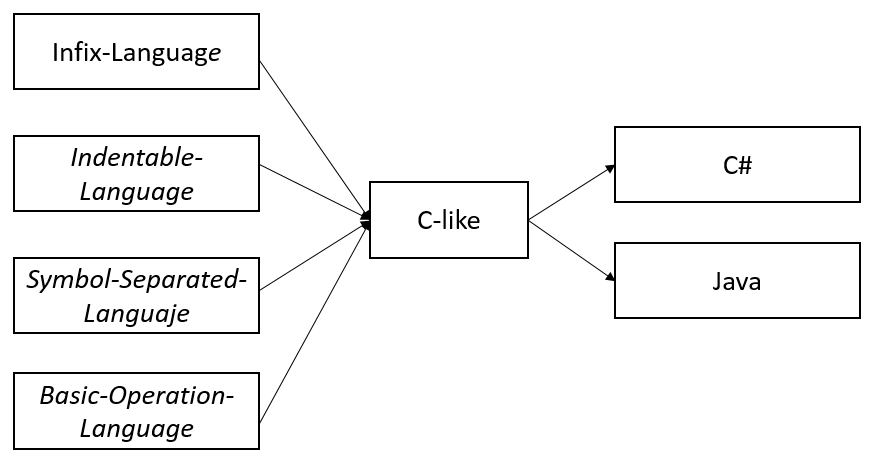
\includegraphics[width=0.6\textwidth]{Adol-jerarquia.png}
	\caption{Jerarquía de lenguajes.}
	\label{Adol8}
\end{figure}

En este capítulo se presentaron las ideas fundamentales para implementar un Generador Multilenguaje en Common Lisp utilizando los macros \texttt{defnode} y \texttt{gcode}. En el próximo capítulo se presentan los principales recursos que permiten cambiar la estructura del código generado por dichos macros. Además se presentan las ideas que permiten automatizar características sintácticas  de los lenguajes de salida.
  

